\section{Billingsley Section 1}
[Berkeley 202a]
[Billingsley - Probability \& Measure]

Why does he say ``closed under countable unions and intersections.​''?

  Billingsley p.19:
  \begin{quote}
    ...require a collection that contains the intervals and is closed under countable unions and intersections.
    Note that a singleton $\{x\}$ is a countable intersection of intervals:
    \begin{align*}
      \bigcap_{n=1}^\infty \Big(x -\frac{1}{n}, x\Big] = \{x\}.
    \end{align*}
  \end{quote}


\begin{itemize}
\item $\Omega = [0, 1]$
\item $\om \in \Omega$
\item $d_n(\om) \in \{0, 1\} = $ $n$-th digit in binary expansion of $\om$
\item Rademacher function $r_n(\om) = 2d_n(\om) - 1 \in \{-1, 1\}$
\end{itemize}

\subsection{Weak Law of Large Numbers}

Define the partial sum $s_n(\om) = \sum_{i=1}^n r_i(\om)$, i.e. the number of $1$s minus the number of $0$s in
the first $n$ digits of the binary expansion of $\om$. (The displacement of the random walk after $n$ steps.)

\begin{lemma}
  \begin{align*}
    \int_0^1 s_n(\om)^2 \d\om = n
  \end{align*}
\end{lemma}

I.e., viewed as a sequence of $n$ coin tosses yielding $-1$ or $+1$, the variance (expected squared distance
from mean) of their sum is $n$.

\begin{proof}
  Note that $s_n(\om)^2 = \sum_{i=1}^n r_i(\om)^2 - 2\sum_{i<j}r_i(\om)r_j(\om)$. Integrating over $[0, 1]$ we have
  \begin{align*}
    \int_0^1 s_n(\om)^2 \d\om
    &= \sum_{i=1}^n \int_0^1 r_i(\om)^2 \d\om - 2\sum_{i<j}\int_0^1r_i(\om)r_j(\om) \d\om \\
    &= \sum_{i=1}^n \int_0^1 1 \d\om - 0 \\
    &= n.
  \end{align*}
  We used there the fact that $\int_0^1r_i(\om)r_j(\om) \d\om = 0$ for $i < j$, i.e that the Rademacher
  functions are orthogonal. An argument for this is that as we move through a rank $i$ dyadic
  interval, $r_i(\omega)$ is constant (either $-1$ or $+1$) while at rank $j$ below, $r_j(\omega)$ flickers
  between $-1$ and $+1$, spending an equal amount of time in each.
\end{proof}


\begin{lemma}[Markov's Inequality]
  Let $f: [0, 1] \to \R^+$ be a step function. Then
  \begin{align*}
    P\Big(\Big\{x: f(x) \geq \alpha\Big\}\Big) \leq \frac{1}{\alpha}\int_0^1 f(x) \dx.
  \end{align*}
\end{lemma}




\begin{intuition}
  Think of the statement in rearranged form:
  \begin{align*}
    \alpha P\Big(\Big\{x: f(x) \geq \alpha\Big\}\Big) \leq \int_0^1 f(x) \dx.
  \end{align*}



  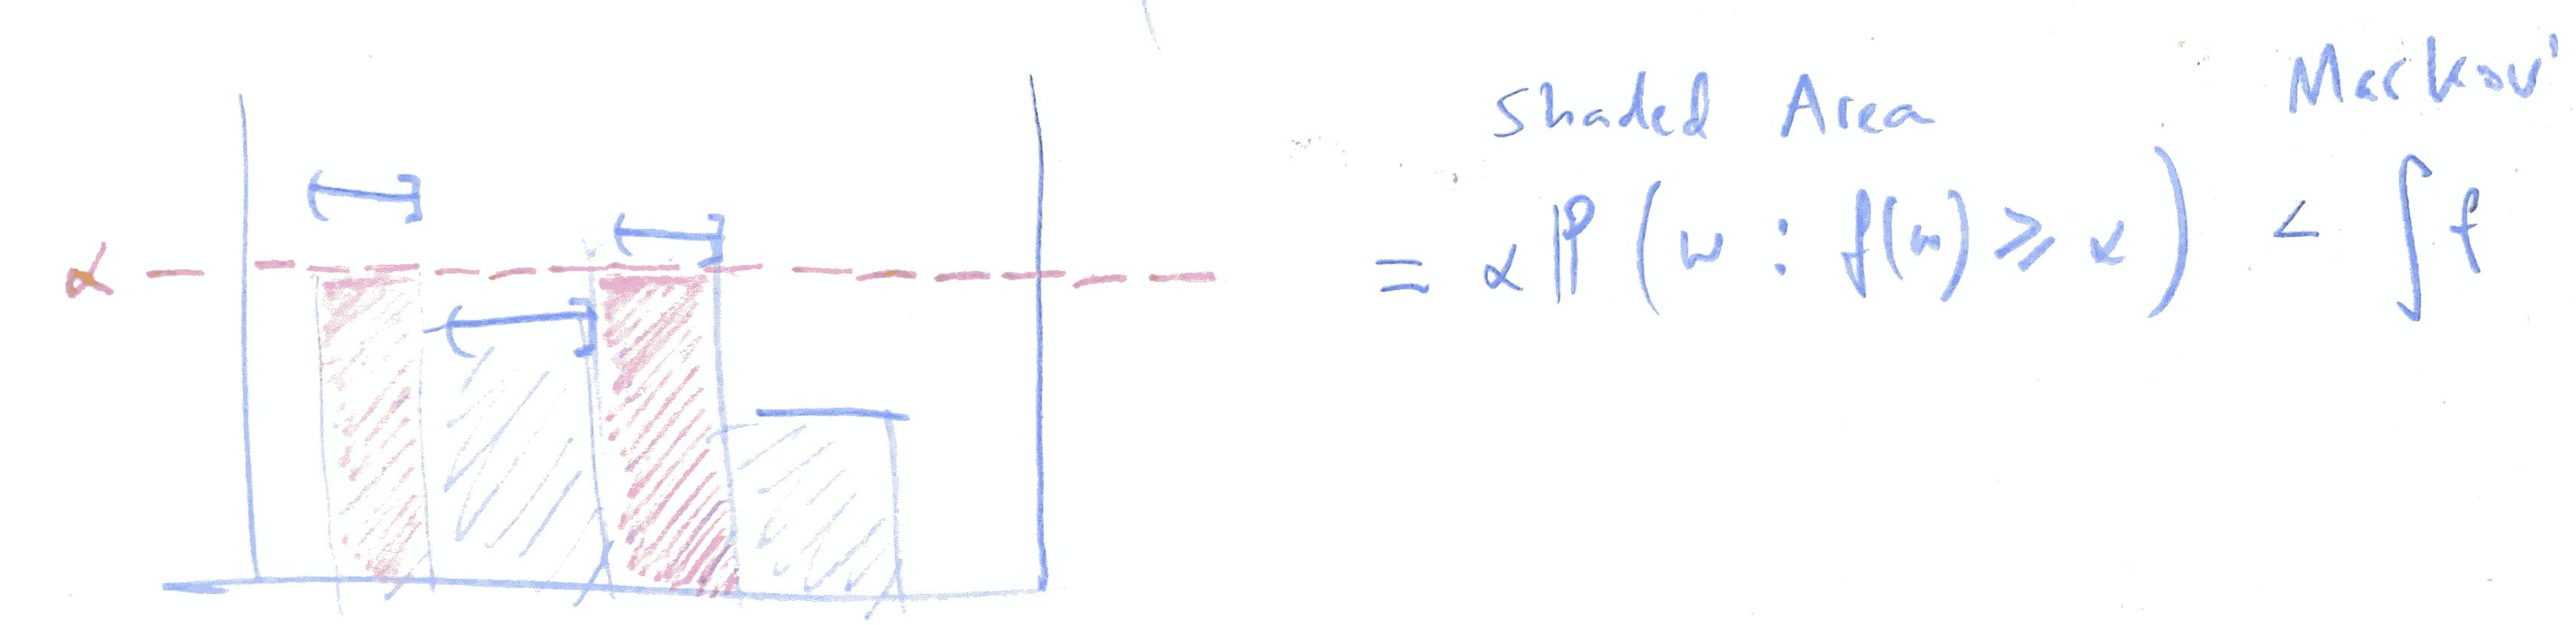
\includegraphics[width=400pt]{img/analysis--real-analysis--measure-theory--weak-law-of-large-numbers-c9c2.png}

  If $X \sim \Unif(0, 1)$ then the RHS is $\E[X]$.

\end{intuition}


\begin{proof}
  [me]

  Clearly
  \begin{align*}
    \int_{f(x) \geq \alpha} f \leq \int_{[0, 1]} f.
  \end{align*}
  Therefore
  \begin{align*}
    \int_{f(x) \geq \alpha} \alpha \leq \int_{[0, 1]} f
  \end{align*},
  or equivalently
\begin{align*}
  \alpha \int \textbf{1}_{f(x) \geq \alpha} \leq \int_{[0, 1]} f,
\end{align*}
which is the same thing as
  \begin{align*}
    \alpha P\Big(\Big\{x: f(x) \geq \alpha\Big\}\Big) < \int_0^1 f(x) \dx.
  \end{align*}
\end{proof}

\begin{theorem}[Weak Law of Large Numbers]
  Fix an $\epsilon > 0$. Then
  \begin{align*}
    \lim_{n \to \infty}P\Big(\Big\{\om: \frac{1}{n}\big|\sum_{i=1}^n r_i(\om)\big| \geq \epsilon\Big\}\Big) = 0.
  \end{align*}
\end{theorem}

In other words: we move through all the $\om \in [0, 1]$. For a given $\om \in [0, 1]$, compare the number
of $0$s and $1$s in the first $n$ digits of the binary expansion, and record the excess as a proportion of $n$;
this is $\frac{1}{n}|s_n(\om)|$. The theorem states that for all $\epsilon > 0$ the probability measure
associated with the set of $\om$s for which $\frac{1}{n}|s_n(\om)| > \epsilon$ goes to $0$ as $n \to \infty$.

\begin{proof}
  Fix an $\epsilon > 0$. We square both sides of the inequality, instead of working with the absolute value. So
  what we want to show is that $P\big(\big\{\om: s_n^2(\om) \geq n^2\epsilon^2\big\}\big) \to 0$
  as $n \to \infty$.

  It would be nice to find an expression for this probability measure as a function of $n$. However, what we'll
  do is find an upper bound: that will suffice also.

  Note that $s_n(\om)$ is a step function (and so $s_n^2(\om)$ is also):

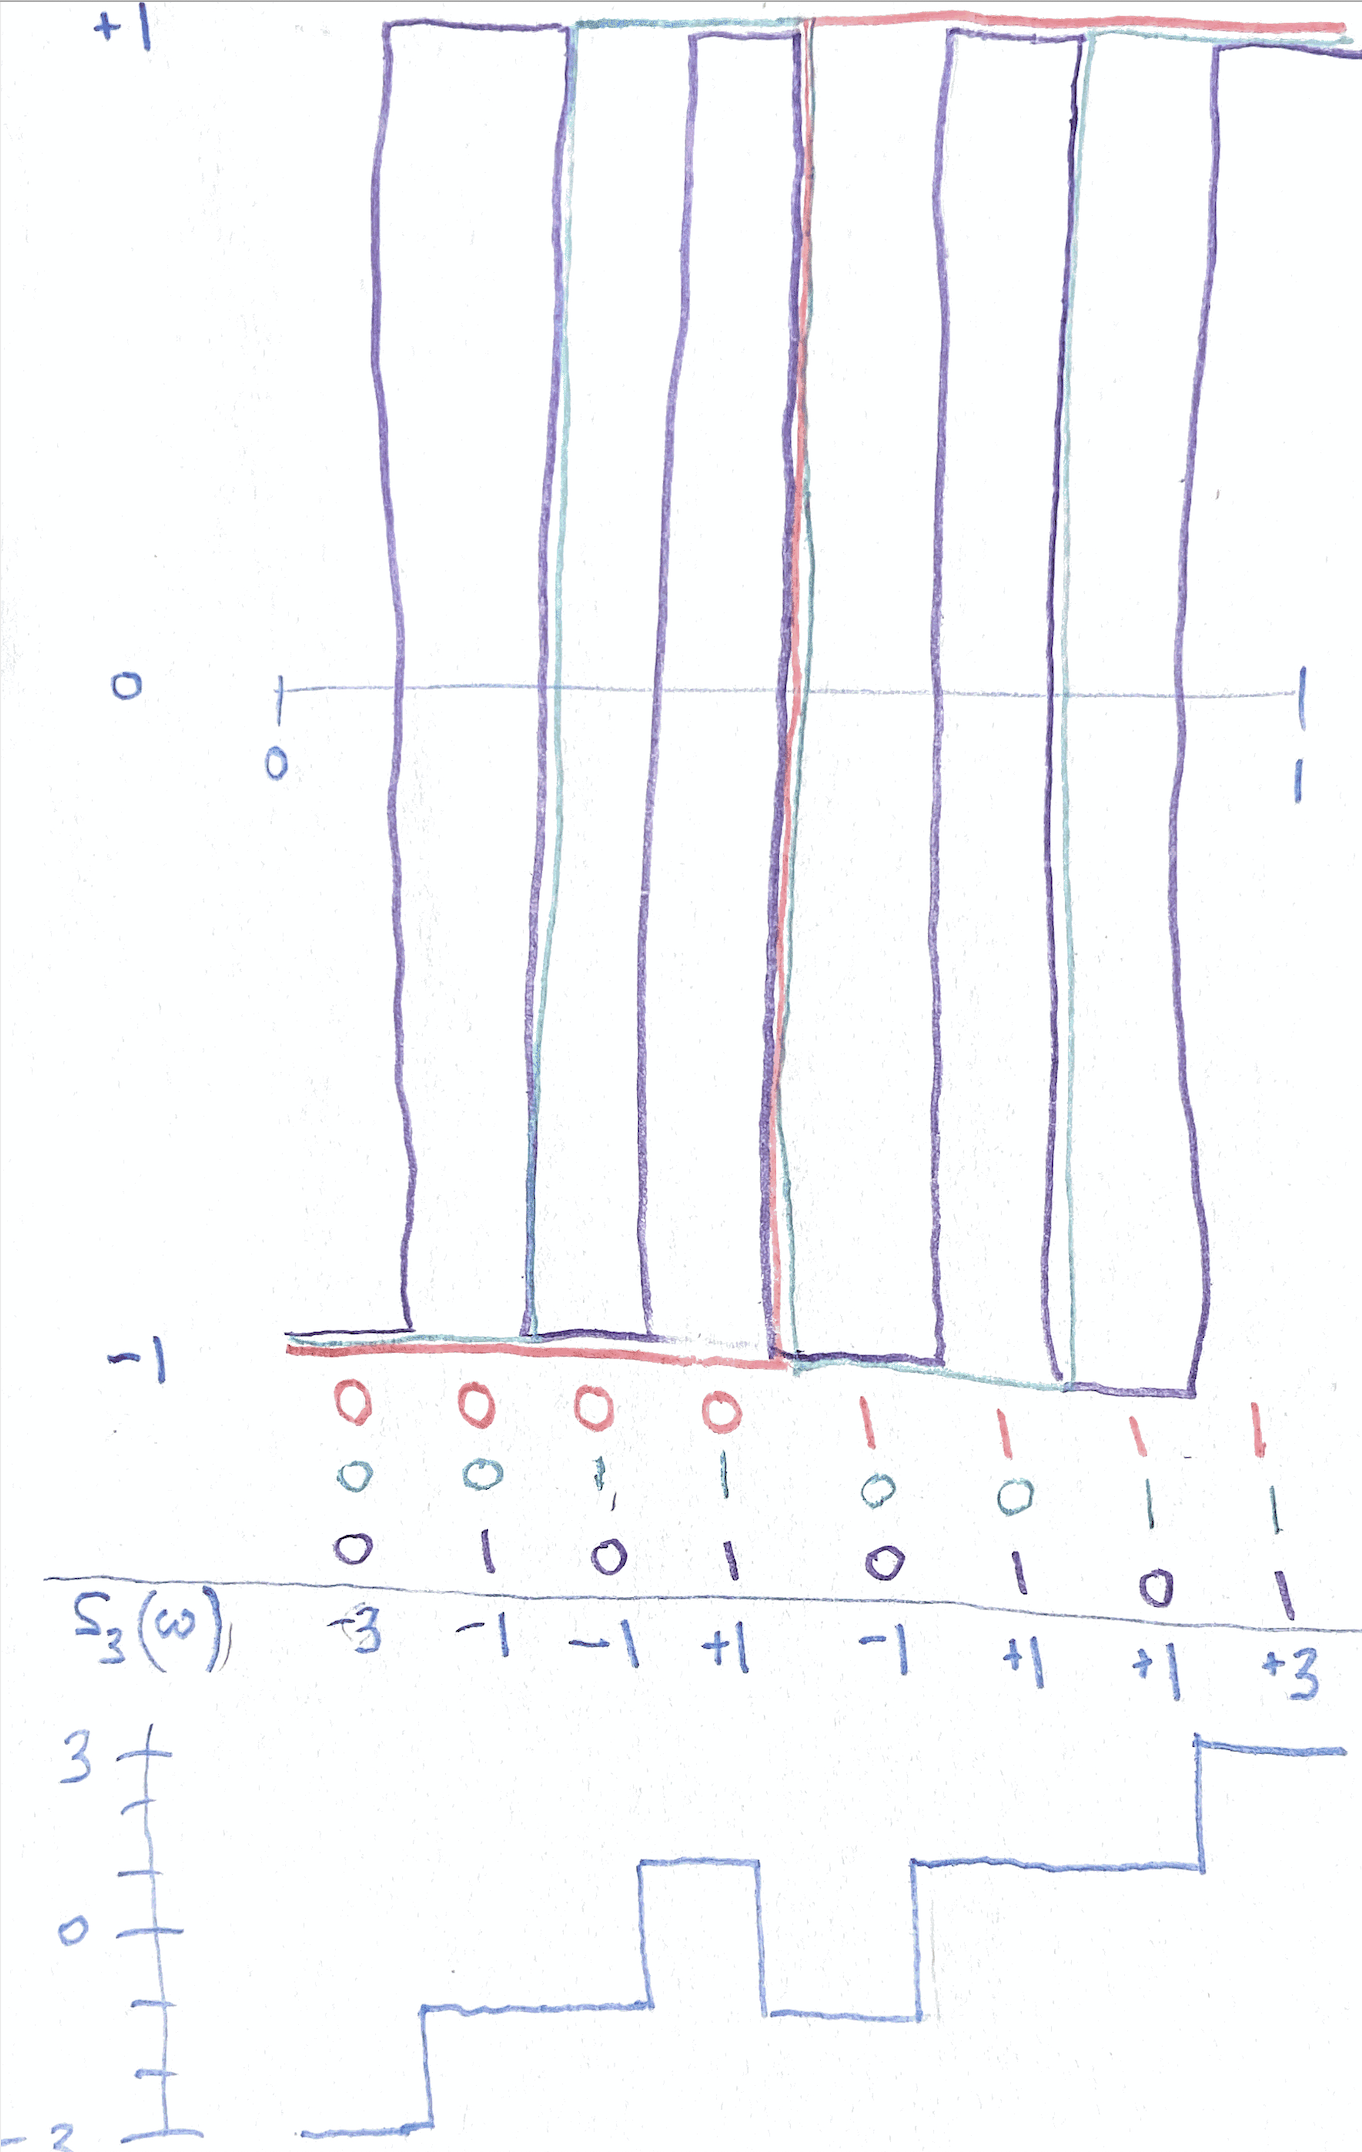
\includegraphics[width=200pt]{img/analysis--real-analysis--measure-theory--weak-law-of-large-numbers-c049.png}


By Markov's inequality / ``Shaded Area lemma​'' we have
\begin{align*}
  n^2\epsilon^2P\Big(\Big\{\om: s_n^2(\om) \geq n^2\epsilon^2\Big\}\Big) \leq \int_0^1 s_n^2(\om) \d\om = n
\end{align*}
and therefore
\begin{align*}
  P\Big(\Big\{\om: s_n^2(\om) \geq n^2\epsilon^2\Big\}\Big) \leq  \frac{1}{n\epsilon^2},
\end{align*}
which proves the desired result since it shows that the probability measure is bounded above by a quantity that
goes to $0$ as $n \to \infty$.
\end{proof}

\subsection{Strong Law of Large Numbers}

\red{TODO} Relation of Borel's normal number theorem to SLNN.

\begin{definition}[negligible, null set]
  A set $A$ is \defn{negligible} if, for any $\epsilon > 0$, it can be covered by a finite or countable
  union $\bigcup_k I_k$ of intervals with $\sum_k |I_k| < \epsilon$.
\end{definition}

Recall the weak law of large numbers:
  \begin{align*}
    \lim_{n \to \infty}P\Big(\Big\{\om: \frac{1}{n}\big|s_n(\om)\big| \geq \epsilon\Big\}\Big) = 0.
  \end{align*}

\begin{definition}[Normal numbers]
  Define the set of \defn{normal numbers} to be
  \begin{align*}
    N = \Big\{\om ~:~ \lim_{n\to\infty} \frac{1}{n}s_n(\om) = 0 \Big\}.
  \end{align*}
\end{definition}

\begin{theorem*}[Borel's normal number theorem]
  $N^c = \R \setminus N$ is negligible.
\end{theorem*}

\begin{intuition}
  Note that the set of normal $\om$ can be written as the set of $\om$ that

  ``eventually stay within $1$​'' AND
  ``eventually stay within $1/2$'' AND
  ``eventually stay within $1/3$'' AND
  ``eventually stay within $1/4$'' ...
  \begin{align*}
    N = \bigcap_{k=1}^\infty \bigcup_{m=1}^\infty\bigcap_{n \geq m} \big\{ \om ~:~ \big|\frac{1}{n}S_n(\om)\big| < \frac{1}{k} \big\}.
  \end{align*}

  Visualize the $s_n$ sequence of a non-normal number $\om$, stretching off to infinity. However far we’ve
  gone, there will always be another point further along at which an excursion of the random walk sticks out
  further than $\eps$. But despite the fact that this must always happen, it’s less and less likely the further
  we go. The fact that it must always happen again corresponds to the fact that we can write the event as a
  countable union: (happened by this generation) union with (happened at the next generation), etc. But at the
  same time, since it’s getting harder and harder, for any given $\gamma >0$ we can find some generation $m$
  beyond which the union sums to less than $\gamma$. nevertheless , the event is equal to the union beyond that
  point, since the departures must always keep occurring (otherwise the number would be normal). So the union
  doesn’t have to include earlier generations.

  This is why the complement of the normal numbers is negligible. Perhaps it’s typical of negligible sets that
  they correspond to an event that must always occur one more time, and yet get ever less and less likely?
\end{intuition}

\begin{proof}
  Let $(\eps_n)$ be a sequence that converges to zero, and define a sequence of sets $(A_n)$, where
  \begin{align*}
    A_n = \Big\{\om : \Big|\frac{1}{n} s_n(\om)\Big| \geq \eps_n\Big\}.
  \end{align*}
  (We can think of $A_n$ as the set of $\om$ whose binary expansions are ``not normal so far​''.)

  Note that, for any given $m$, we have the following: a number that stays inside $\eps_n$ for ever is normal:
  \begin{align*}
    \Big(\bigcap_{n=m}^\infty A_n^c\Big) \subset N.
  \end{align*}
  Equivalently, a non-normal number must stray outside $\eps_n$ at some point:
  \begin{align*}
    N^c \subset \Big(\bigcup_{n=m}^\infty A_n\Big).
  \end{align*}
  Recall that our aim is to cover $N^c$ with a countable union of intervals, where the total length of the
  intervals is arbitrarily small (an ``efficent covering​​''). If we can show that the $A_n$ meet that
  description then we are done.

  Recall that $s_n$ is a step function such that, if $\om \in A_n$ then $\om' \in A_n$ for every $\om'$ in the
  same rank-$n$ dyadic interval as $\om$. Therefore each set $A_n$ is a finite disjoint
  union $\bigcup_{k}I_{nk}$ of intervals, and $P(A_n) = \sum_k |I_{nk}|$.

  So what we need to do is show that, for any given $\gamma > 0$, there exists a sequence $(\eps_n)$ converging
  to zero, and an $m$, such that $\sum_{n=m}^\infty P(A_n) < \gamma$.

  At this point, we need to find an expression for an upper bound on $P(A_n)$ in terms of $n$ and $\eps_n$.
  From the lemma, we have
  \begin{align*}
    P(A_n) \leq \frac{3}{n^2\eps_n^4},
  \end{align*}
  so we would like to find $(\eps_n)$ and $m$ such that
  \begin{align*}
    \sum_{n=m}^\infty \frac{3}{n^2\eps_n^4} < \gamma.
  \end{align*}
  To do so, we need only choose $(\eps_n)$ so that the series $\sum_nn^{-2}\eps_n^{-4}$
  converges: $\eps_n = n^{-1/8}$ will do. Then, since the series converges, there exists an $m$ such that the
  tail sums to less than $\gamma$, as required.
\end{proof}

\begin{lemma}
  Let $A_n = \Big\{\om : \Big|\frac{1}{n} s_n(\om)\Big| \geq \eps\Big\}$.

  For all $n \in \N$, we have (by taking the 4th power of both sides of the inequality and applying Markov's
  inequality)
  \begin{align*}
    P(A_n) \leq \frac{1}{n^4\eps^4} \int_0^1 s_n^4(\om) \d\om,
  \end{align*}
  and (by considering integrals of products of four Rademacher functions)
  \begin{align*}
    \int_0^1 s_n^4(\om) \d\om \leq 3n^2.
  \end{align*}
  Therefore
  \begin{align*}
    P(A_n) \leq \frac{3}{n^2\eps^4}.
  \end{align*}
\end{lemma}

\newpage
\subsection{An interval of  positive length is not negligible}

\begin{definition*}[length of an interval]
  The \defn{length} of $(a, b)$ is $|(a, b)| = b - a$.
\end{definition*}

\begin{theorem*}
  Let $I$ be an interval of positive length and let $I_1, I_2, \ldots$ be intervals.
  \begin{enumerate}
  \item If $\bigcup_k I_k \subseteq I$ (disjoint) then $\sum_k |I_k| \leq |I|$
  \item If $\bigcup_k I_k \supseteq I$ then $\sum_k |I_k| \geq |I|$. I.e. no cover of $I$ is negligible.
  \end{enumerate}
  A corollary is that if $\bigcup_k I_k = I$ then $\sum_k |I_k| = |I|$.
\end{theorem*}

\begin{proof}
  Let $I = (a, b)$ and let $I_k = (a_k, b_k)$ for all $k$.

  First, we show that if $\bigcup_k I_k \subseteq I$ (with the $I_k$ disjoint) then $\sum_k |I_k| \leq |I|$.

  There are two cases:
  \begin{enumerate}
  \item {\bf Finite cover}:

    The claim is that for any collection of $n$ disjoint intervals, if $\bigcup_{k=1}^n I_k \subseteq I$
    then $\sum_{k=1}^n |I_k| \leq |I|$.

    This is clearly true for a collection of intervals of size $n = 1$.

    Assume it's true for any collection of intervals of size $n-1$, and consider a collection of $n$ disjoint
    intervals with $\bigcup_{k=1}^n I_k \subseteq I$.

    Label the intervals $I_1, \ldots, I_n$, sorted by their left endpoint in ascending order. Note that the
    union of the first $n-1$ intervals is contained within $(a, a_n)$ and that the $n$-th interval has
    length $b_n - a_n \leq b - a_n$. Thus we have
    \begin{align*}
      \sum_{k=1}^n |I_k|
      &= \sum_{k=1}^{n-1}|I_k| + |I_n| \\
      &\leq (a_n - a) + (b - a_n) \\
      &= b - a.
    \end{align*}
    Therefore it is true for all $n$ by induction.

  \item {\bf Infinite cover}:

    The claim is that for any countably infinite collection of $n$ disjoint intervals,
    if $\bigcup_{k=1}^\infty I_k \subseteq I$ then $\sum_{k=1}^\infty |I_k| \leq |I|$.

    Consider an infinite collection of intervals satisfying $\bigcup_{k=1}^\infty I_k \subseteq I$.

    Note that for every finite subcollection of size $n$ we have $\sum_{k=1}^n |I_k| \leq |I|$ by the finite case.

    Therefore $\sum_{k=1}^\infty |I_k| = \sup \sum_{k=1}^n |I_k| \leq |I|$ where the supremum is over the set
    of all finite subcollections. Since this set is non-empty, the supremum is a finite positive number.
  \end{enumerate}
  ~\\~\\
  Finally, we show that if $\bigcup_k I_k \supseteq I$ then $\sum_k |I_k| \geq |I|$.
  Again, there are two cases:
  \begin{enumerate}
  \item {\bf Finite cover}:

    The claim is that for any collection of $n$ intervals, if $\bigcup_{k=1}^n I_k \supseteq I$
    then $\sum_{k=1}^n |I_k| \geq |I|$.

    In other words, that the total length of a finite cover of $I$ is bounded below by $|I| > 0$.

    Again, it's obvious for a cover comprising a single interval ($n=1$).

    Assume it's true for any cover comprising $n-1$ intervals, and consider a cover comprising $n$ intervals.

    Again, label the intervals $I_1, \ldots, I_n$, sorted by their left endpoint in ascending order.

    Note that the first $n-1$ intervals cover the interval $(a, b_{n-1})$ and that $|I_n| \geq b - b_{n-1}$.
    Thus we have
    \begin{align*}
      \sum_{k=1}^n |I_k|
      &= \sum_{k=1}^{n-1}|I_k| + |I_n| \\
      &\geq (b_{n-1} - a) + (b - b_{n-1}) \\
      &= b - a.
    \end{align*}

  \item {\bf Infinite cover}\\

    The claim is that for any infinite cover $\bigcup_{k=1}^\infty I_k \supseteq I$ we have $\sum_{k=1}^\infty |I_k| \geq |I|$.

    Consider a countably infinite cover of $I$.

    We might think that we could make an argument analogous to the one above:

    Note that for every finite subcover of size $n$ we have $\sum_{k=1}^n |I_k| \geq |I|$.

    Therefore $\sum_{k=1}^\infty |I_k| = \inf \sum_{k=1}^n |I_k|  \geq |I|$ where the infimum is over the set of all finite subcovers.

    However, we have to show that a finite subcover exists; otherwise the infimum would be $+\infty$.

    So what we do is construct a closed interval $[a + \eps, b]$ which is covered by a countably infinite open
    cover. Since that closed interval is compact from Heine-Borel, there exists a finite open subcover.

    \begin{quote}
      I think your second statement is true except for an infinite open cover of (a, b] which has finite total
      measure, but no finite subcovers. Such a cover does exist, and it’s the the object I was (clumsily)
      trying to refer to. So I think your second statement is false, but not nonsense, as it fails for the same
      reason that the second proof is more difficult.
    \end{quote}
  \end{enumerate}
\end{proof}


\begin{theorem}
  Every proper open subset of $\R$ is a countable union of disjoint open intervals and open rays.
\end{theorem}
\begin{proof}
  HW2 Q1 (uses an equivalence relation to partition the open set), Billingsley Example 2.6 (uses an
  uncountable union of intervals with rational endpoints which must contain duplicates).
\end{proof}


\begin{proof}
  Let $\ms A$ be a finite class of $n$ sets. Taking complements gives $2n$ sets.

  In the first iteration, each set can be involved in $2n$ unions and $2n$ intersections, for a total of $4n$
  new sets, which becomes $8n$ on taking complements.

  So after $k$ generations, we


\end{proof}
\subsection{sigma-algebras, Borel sets}

\url{https://en.wikipedia.org/wiki/Outcome_(probability)}


An \defn{outcome} is an atomic, lowest-level, result of an experiment/process. Outcomes are mutually exclusive.

An \defn{event} is a set of \defn{outcomes} that we assign probability to. It is a subset of $\Omega$. Events are not mutually
exclusive: ``greater than 0.5?​'' and ``greater than 0.6?​'' are both events and, for a given outcome, both events
may ``occur​''.

An \defn{algebra} is a collection of events. So an algebra contains all the things we might assign probability to.
Furthermore, an algebra must be closed under complementation, union and intersection ( ``not​'', ``or​'', and ``and​'').

A $\sigma$-\defn{algebra} is an algebra that is closed under countably infinite unions and intersections.

\begin{theorem}
  An open set is a {\it countable} union of disjoint intervals.
\end{theorem}

\begin{definition*}[$\sigma$-algebra]
  An \defn{algebra} in $\Omega$ is a collection of subsets of $\Omega$ that
  \begin{enumerate}
  \item contains $\emptyset$ and $\Omega$
  \item is closed under complements
  \item is closed under {\it finite} unions and intersections
  \end{enumerate}

  It is a $\sigma$-\defn{algebra} if it is additionally closed under {\it countable} unions and intersections.
\end{definition*}

\begin{definition}
  A ($\sigma$-) algebra \defn{generated} by a collection of subsets is the smallest ($\sigma$-) algebra of which that
  collection is a subset.
\end{definition}


\begin{quote}
  the intersection of all fields in $\Omega$ containing $\ms A$.
\end{quote}

Here, ``containing​'' means subset inclusion.

An in fact, ``in​'' here means neither set membership nor subset inclusion. It is used in a more technical sense
to refer to fields whose sets are subsets of $\Omega$ (i.e. fields that are elements of the powerset
of $\Omega$). Bass uses ``on​'' for this: ``a field on $\Omega$​''.

\begin{definition}[Borel $\sigma$-algebra, Borel set]
  A \defn{Borel} $\sigma$-\defn{algebra} is the $\sigma$-algebra generated by the open sets.

  A \defn{Borel set} is a subset of $\Omega$ that is an element of a Borel $\sigma$-algebra.
\end{definition}

A Borel $\sigma$-algebra contains is generated by open sets (and so equivalently by closed sets). But
the $\sigma$-algebra contains singletons, half-closed intervals, etc.

\begin{theorem}
  The Borel $\sigma$-algebra on $\R$ can be generated by the following sets
  \begin{enumerate}
  \item $\ms I_1 = \{(a, b) ~:~ a, b \in \R\}$
  \item $\ms I_2 = \{[a, b] ~:~ a, b \in \R\}$
  \item $\ms I_3 = \{(a, b] ~:~ a, b \in \R\}$
  \item $\ms I_4 = \{[a, \infty) ~:~ a \in \R\}$
  \item $\ms I_5 = \{(p, q) ~:~ p, q \in \Q\}$
  \end{enumerate}
\end{theorem}

\begin{proof}
  Let $\ms O$ be the collection of open subsets of $\R$, so that $\ms B = \sigma(\ms O)$.
  \begin{enumerate}
  \item The key here is that every open subset of $\R$ is a countable union of open intervals. So the collection of
    open sets is automatically in the $\sigma$-algebra generated by the open intervals, so you can't ``get
    anything new​'' from them.

    Let $\ms I_1 = \{(a, b) ~:~ a, b \in \R\}$. We want to show that $\sigma(\ms I_1) = \sigma(\ms O)$.

    In one direction, every element of $\ms I_1$ is open, so clearly $\sigma(\ms I_1) \subseteq \sigma(\ms O)$.

    For the other direction, let $X \in \ms O$ be an open subset of $\R$. Then $X$ is a countable union of open
    intervals (i.e. finite intervals and open rays). Every finite interval is in $\ms I_1$. But open ray are
    also countable unions of finite intervals: $(-\infty, a) = \bigcup_n^\infty (a-n, a)$
    and $(a, \infty) = \bigcup_n^\infty (a, a + n)$. Therefore $X \in \sigma(\ms I_1)$, i.e. every open set is
    in the $\sigma$-algebra generated by open intervals. This is equivalent to the
    statement $\ms O \subseteq \sigma(\ms I_1)$, i.e. the collection of all open sets is a subset of
    that $\sigma$-algebra. Therefore $\sigma(\ms O) \subseteq \sigma(\sigma(\ms I_1)) = \sigma(\ms I_1)$.

  \item We reduce this to (1) by showing that we can make $(a, b)$ from $[a, b]$.

    Let $\ms I_2 = \{[a, b] ~:~ a, b \in \R\}$. We want to show that $\sigma(\ms I_2) = \sigma(\ms O)$.

    To show $\sigma(\ms I_2) \subseteq \sigma(\ms O)$, note that for $a < b$
    \begin{align*}
      [a, b] &= \bigcap_{n=1}^\infty (a - n^{-1}, b + n^{-1}).
    \end{align*}
    Therefore $[a, b] \in \sigma(\ms I_1)$ for all $a, b \in \R$, hence $\sigma(\ms I_2) \subseteq \sigma(\ms I_1) = \sigma(\ms O)$.

    To show $\sigma(\ms O) \subseteq \sigma(\ms I_2)$, note that for $a < b$ and $n_0 \geq 2/(b - a)$
    \begin{align*}
      (a, b) &= \bigcup_{n=N_0}^\infty [a + n^{-1}, b - n^{-1}].
    \end{align*}
    Therefore $(a, b) \in \sigma(\ms I_2)$ for all $a, b \in \R$ hence $\ms I_1 \subseteq \sigma(\ms I_2)$,
    hence $\sigma(\ms I_1) = \sigma(\ms O) \subseteq \sigma(\ms I_2)$. But we have already shown
    that$\sigma(\ms I_1) = \sigma(\ms O)$, therefore $\sigma(\ms O) \subseteq \sigma(\ms I_2)$.
  \end{enumerate}
\end{proof}

\subsection{Bass 3. Measures}

Let $\Omega$ be a set and $\mc A$ a $\sigma$-algebra on $\Omega$.

A \defn{measure} is a function $\mu:\mc A \to [0, \infty]$ that is \defn{countably additive} (CA; measure of disjoint union equals sum of measures).

CA has various implications which make $\mu$ behave in unsurprising ways:
\begin{enumerate}
\item It's finitely and countably \defn{subadditive} (measure of union does not exceed sum of measures)
\item Measure of limiting sets equals limit of measures (e.g. if $A_i \uparrow A$ then $\mu(A) = \lim_n \mu(A_i)$)
\end{enumerate}

\begin{intuition*}
  The function $\mu$ is a map from sets to reals. So in principle it could assign whatever real values it wants
  to whatever sets. E.g. for disjoint $A, B$ it could assign a value to $\mu(A \cup B)$ that is completely
  different from $\mu(A) + \mu(B)$.

  In fact, however, measures treat sets as an aggregate of points. I think that everything is perfectly
  intuitive except that countably infinite unions might not work as expected.

  In other words, $\mu$ acts exactly as one would expect: as if it's applying a uniform layer of paint to each
  subset: the total amount of paint used to paint a union of disjoint sets is the sum of the paint applied to
  each set in the union.

  But CA means the additivity is retained even when there are infinitely many sets in the union. An example of CA
  failing to hold is densities of finite subsets of the natural numbers: the density of the singleton $\{1\}$ as
  a proportion of the natural numbers is naturally defined to be $0$ (the limit of the density in a finite sample
  as the sample size tends to infinity). But the density of the countable union of all singletons is $1$, which is
  not the sum of the densities.
\end{intuition*}

A measure is \defn{finite} if $\mu(\Omega) < \infty$, and $\sigma$\defn{-finite} if there exists a countable partition
of $\Omega$ with each subset in the partition having finite measure.

$(\Omega, \mc A, \mu)$ is a \defn{measure space}.

A subset $A \subset \Omega$ (not necessarily in $\mc A$) is a \defn{null set} if $A$ is a subset of some element
of $\mc A$ which has zero measure. $(\Omega, \mc A, \mu)$ is a \defn{complete} measure space if all null sets are
in $\mc A$. The \defn{completion} of $\mc A$ is the smallest complete $\sigma$-algebra $\bar{\mc A}$ containing
$\mc A$ such that $(\Omega, \bar{\mc A}, \bar \mu)$ is a complete measure space, where $\bar \mu$ is an
extension of $\mu$ from $\mc A$ to $\bar{\mc A}$.

A \defn{probability measure} is a measure where $\mu(\Omega) = 1$.

\subsection{Bass 4.  Construction of measures}

\subsubsection{Overview}

\begin{enumerate}

\item We want a function that, in some appropriate sense, measures the {\it length} of an arbitrary subset of
  $\R$.

\item We're not going to get the ``sensible measure of length​'' property out of nowhere: we're going to inject a
  pre-existing sensible measure of length of tractable sets at a low level, and build on this.

\item That low-level ``sensible measure of length​'' is, when we're working with $\R$, going to be the length of an
  interval: $|(a, b)| = b - a$.

\item Clearly we want our measure of length to be additive over a finite collection of subsets. But we will also
  require it to be additive over a countably infinite collection of subsets, and this requirement is central to
  everything that follows.

\item So, more precisely, what we want is a {\it countably additive} set function (i.e. a \defn{measure}) defined on a large collection (as
  large as possible) of subsets of $\R$, that is a ``sensible measure of length​'' of those subsets.

\item A theorem tells us a way to make a {\it countably sub-additive} set function (i.e. an \defn{outer measure}) defined on {\it all} subsets:
  \begin{enumerate}
  \item Let $E$ be an arbitrary subset of $\R$ that we want to measure.
  \item Now, restrict attention to the collection of ``low-level​'' subsets of $\R$ for which we have the pre-existing
    sensible measure of length. In $\R$, these are open intervals, or perhaps half-open intervals \red{open sets?}.
  \item Sometimes, one of these low-level subsets will cover $E$. But if $E$ is not a simple interval, we will
    approximate the length of $E$ better with a collection of low-level subsets whose union covers $E$, while
    none of them do on their own. Whether it is a collection of one or many, we will refer to this as a
    ``covering collection of subsets​''.
  \item Note that the covering collection is built out of the low-level subsets, so we can assign a sensible
    measure of length to the covering collection: in $\R$, it is just the sum of lengths of the intervals involved.
  \item Create a set containing the measure of every covering collection. We define our outer measure on $E$ to be
    the infimum (greatest lower bound) of that set. Roughly speaking, we've defined $\mu^*(E)$ to be the total
    length of the collection of intervals that cover $E$ most efficiently (with least unnecessary overlap).
  \end{enumerate}

\item We will call our outer measure $\mu^*$. Clearly it is a reasonable measure of length for some sets.

\item Recall that it is defined on {\it all} subsets of $\R$ (its definition involved our restricted collection of
  ``low-level​'' subsets, but the resulting procedure can be applied to any subset).

\item Pause here: this definition of $\mu^*$ is fundamental. The outer measure that we assign to an arbitrary
  subset $E$ is obtained by using the intervals $I_i$ that we {\it can} measure. We look over all collections of
  the $I_i$ that cover $E$ and record the total length of each cover. The infimum of these cover lengths is the
  measure assigned to $E$:
  \begin{align*}
    \mu^*(E) = \inf\Big\{\sum_i \ell(I_i) : E \subseteq \bigcup_i I_i\Big\}.
  \end{align*}
\item Now, it's nice that it is defined on all subsets of $\R$, and it does have some sensible properties such as
  countable sub-additivity, and probably finite additivity, but it does {\it not} necessarily have the countable
  additivity property that we require.

\item We can get that though with an adjustment: we restrict the collection of subsets that we're allowed to
  measure, so that it's no longer {\it all} subsets.

\item There are two candidates we could restrict to. One is the \defn{Borel} $\sigma$-algebra. This is the
  $\sigma$-algebra generated by the open subsets.

\item However, there's a larger $\sigma$-algebra we can restrict to: the \defn{Lebesgue} $\sigma$-algebra. This is the class
  of $\mu^*$-measurable sets. A set $A \subset \R$ is $\mu^*$-measurable if finite additivity holds between $A$
  and every other subset of $\R$, that is $\mu^*(A \cap E) + \mu^*(A \cap E^c) = \mu^*(A)$ for
  all $E \subset \R$.

\item The Borel $\sigma$-algebra is contained within the Lebesgue $\sigma$-algebra. Restricting $\mu^*$ to either
  gives us what we want: countable additivity. The restriction of $\mu^*$ to the Lebesgue $\sigma$-algebra is
  \defn{Lebesgue measure} $\mu$.

\item The above involved using interval length as our measure of the low-level subsets:
  $\ell(I_i) = b_i - a_i$. There is an important generalization known as \defn{Lebesgue-Stieltjes measure}: we introduce a
  real-valued increasing function $\alpha: \R \to \R$ that distorts the measures we assign to each
  interval: $\ell(I_i) = \alpha(b_i) - \alpha(a_i)$. So an interval in a region in which $\alpha$ is increasing
  rapidly has larger measure. Other than that, the theory for Lebesgue-Stieltjes measure is the same: we define
  the outer measure using the low-level intervals on which $\ell$ is defined, and we restrict to the collection
  of measurable sets, which is a $\sigma$-algebra.

\end{enumerate}


Suppose we are defining a measure $m$ on $\Omega = \R$.

Since an open set $G$ is a countable union of disjoint open intervals, we want
\begin{align*}
  m(G) = \sum_{i=1}^\infty b_i - a_i.
\end{align*}
The basic idea is that, for a set $E$, we are going to define $m(E)$ to be the measure of the smallest open
cover of $E$:
\begin{align*}
  m(E) := \inf \{ m(G) ~:~ G \text{~open~}, E \subseteq G\}.
\end{align*}
However, the infimum has to be restricted to a $\sigma$-algebra that is smaller than all subsets of $\R$ (the
latter is a $\sigma$-algebra, but it's not possible to construct a measure with this as its domain [theorem]).

An \defn{outer measure} is defined similarly to a measure. The difference is
\begin{enumerate}
\item It is defined on {\it all} subsets of $\Omega$
\item It obeys \defn{countable subadditivity}, but {\it not} necessarily countable additivity.
\end{enumerate}

A common way to construct an outer measure is
\begin{enumerate}
\item Define a collection $\mc C$ of subsets of $\Om$ (the collection must contain a subset that partitions $\Om$.)
\item Define a cost function $\ell : \mc C \to [0, \infty]$
\item Define $\mu^*(E)$ to be the cost of the least-cost cover of $E$:
  \begin{align*}
    \mu^*(E) := \inf \Big\{\sum_{i=1}^\infty\ell(C_i) ~:~ E \subseteq \bigcup_{i=1}^\infty C_i\Big\}.
  \end{align*}
  Note what this does: it defines $\mu^*$ on {\it any} subset $E$, while the collection $\mc C$ typically comes from a
  restricted collection (e.g. open sets).
\end{enumerate}

It's obvious that this is FSA but one has to prove that it is CSA (using an epsilon-of-room technique).

\begin{question*}
  \red{TODO} Must an outer measure be finitely additive?

  I don't think so, FA doesn't follow from CS. But could one include FA in the definition of an outer measure?


Is an outer measure always FA? I.e. the issue is just getting CA?

=> Sort of but look at Vitali construction for a counter-example

  Is the (canonical) example given finitely additive?
\end{question*}

\begin{example}[Lebesgue measure on subsets of $\R$]
  \begin{enumerate}
  \item Consider the collection of all open intervals $O \subseteq \R$.
  \item Define $\ell(O)$ in the normal way (sum of $b_i - a_i$ over the disjoint open intervals).
  \item Define $\mu^*(E)$ to be the infimal cost of an open cover of $E$ (i.e. as above in the canonical
    construction of outer measure)
  \end{enumerate}
  So what we've just constructed is an outer measure: it assigns a measure to {\it any} subset $E$, using open sets
  for the cover.

  It must be countably sub-additive, because it used the canonical construction, and we have a theorem for that.

  Now, we would ideally like this to be a measure on all subsets of $\R$, i.e. countably additive.

  It isn't (theorem), but it {\it is} a measure on a restricted collection of subsets of $\R$. That collection is
  the $\sigma$-algebra generated by the open sets (the Borel algebra).

  This measure is \defn{Lebesgue measure}.

  To recap: it was constructed as follows:
  \begin{enumerate}
  \item We want to assign a value to some subset $E$
  \item We use open intervals to cover $E$
  \item The value assigned to $E$ is the measure of the smallest open cover (using length of open intervals to
    define measure here)
  \item This gives a countably subadditive function (an outer measure).
  \item But this is only countably additive for $E$ in the $\sigma$-algebra.
  \end{enumerate}
\end{example}

\begin{intuition*}
  Outer measures have that name because they approximate from above ( ``shrink-wrapping​'').

  When you approximate from above, you get something which is countably subadditive:

  \begin{proof}
    Suppose $\mu^*(A \cup B) > \mu^*(A) + \mu^*(B)$.

    Intuitively, take the most efficient cover of $A$ and the most efficient cover of $B$. Their combined cost
    is $\mu^*(A) + \mu^*(B)$. But together they are a cover of $A \cup B$. But that implies that the most
    efficient cover of $A \cup B$ is no greater than $\mu^*(A) + \mu^*(B)$; a contradiction.

    A real proof has to deal with the fact that we're dealing with infima, not minima.
  \end{proof}
\end{intuition*}
